\let\textcircled=\pgftextcircled
\chapter{Holistic Project Map}
\label{chap:map}

\initial{T}he project is a collaboration of separate parts to form a fully functional whole. While this paper focuses on the sensory apparatus and data interpretation, it is worth noting how it links to the other work taking place providing further functionality to the drone. Figure \ref{fig:map} describes the relationship between these component pieces.

\begin{figure}
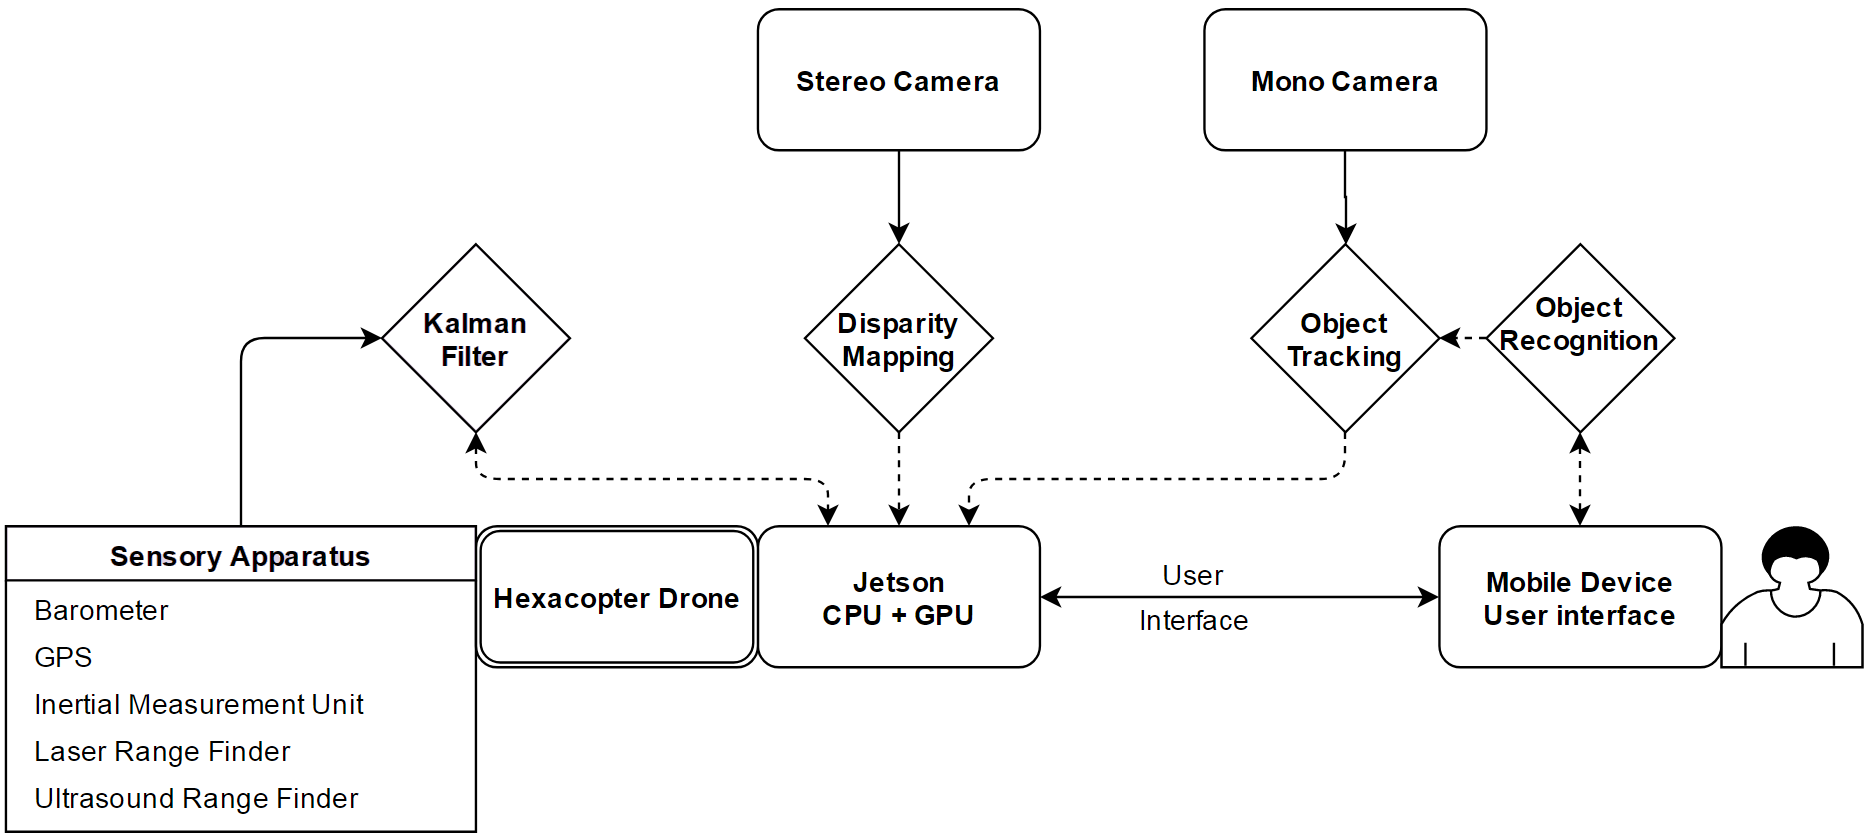
\includegraphics[width=\textwidth]{largeprojectdiagramwhite.png}
\mycaption[Project Diagram]{Project Diagram}
\label{fig:map}
\end{figure}

The filter used in this project takes in data from many of these other sections as well as the sensory apparatus described in this paper. Distance to objects is provided by the disparity mapping, and positional/velocity information is relayed from the GPS. Fast and efficient communication between these components is vital and requires coordination between projects.
%=======